\documentclass[a4paper,12pt]{article}

% Required packages
\usepackage[utf8]{inputenc}
\usepackage{graphicx}
\usepackage{geometry}
\usepackage{hyperref}
\usepackage{fontawesome}
\usepackage{amsmath}
\geometry{margin=1in}

\title{Portfolio Project Report}
\author{Your Name}
\date{\today}

\begin{document}

\maketitle
\tableofcontents

\newpage

% Section 1: Introduction
\section{Introduction}
This project aims to develop a complete portfolio that shows my technical skills for the position of a working student. Having a well-structured portfolio is a must in the competitive job market today to show practical skills concerning computer science and web development. This portfolio is meant to expose my web development, technical documentation, and data analysis, which are the most needed during the hiring process of a working student. Along the way, I want to be able to provide potential employers with clear proof of my technical competencies, creativity, and problem-solving skills.
It consists of three key components: a personal website, a LaTeX CV, and an analytics task. The personal website will be maintained in GitHub Pages and will provide a unified platform for the presentation of my academic background, technical skills, and project experience. It's designed to be responsive, professional, and user-friendly. The LaTeX CV is part of the portfolio, showing my skills in using LaTeX to create structured and professional documents, considered one of the most accurate tools in the technical and academic set. Then, the analytics task shows my skills in data analysis through Python by analyzing data, visualizing results, and evaluating the performance of machine learning models using its relevant libraries.
This report is structured to reflect the three major components of the portfolio. First, it will cover the design and structure of the website, focusing on major design decisions, tools, and technologies used. Second, it will look at the LaTeX CV, focusing on its structure and the tools used in its creation. The final section will have the analytics task: what data were used, which tools were used to analyze, actual analysis process, and results. Further on, the report extends to include reflections about the project and what possibly would be improved in subsequent iterations. The structure ensures a logical flow of information within the report.


% Section 2: Portfolio Website
\section{Portfolio Website}

% Subsection 2.1: Website Design and Structure
\subsection{Website Design and Structure}
The portfolio website is an inclusive medium to represent your academic background, projects, and technical skills professionally. This is about achievements and being capable technologically, which will be represented in an easy-to-navigate interface: visitors are potential employers and peers. The main purpose of the website will be an online home that connects multiple skills of computer science, web development, and data analysis into one location. The website uses Bootstrap CSS to ensure a professional look, keeping in mind an up-to-date feel, and focusing on functionality and responsiveness.

% Subsubsection 2.1.1: Pages Overview
\subsubsection{Pages Overview}

\paragraph{Home Page (Who Am I)}
The "Home Page," titled "Who Am I," introduces the visitor to my career goals and personal interests. It was designed using Bootstrap to ensure that clear sections are there, with user-friendly navigation. Visitors will notice immediately my focus areas and objectives. A profile image is included with compact text in an engaging tone to establish a personal touch with the audience. This page represents me excellently by stating my interest in Computer Science, Software Development, and Web Technologies. This is neat and ensures whatever you have on the page is accessible and appealing to create that first impression.

\begin{figure}[h!]
    \centering
    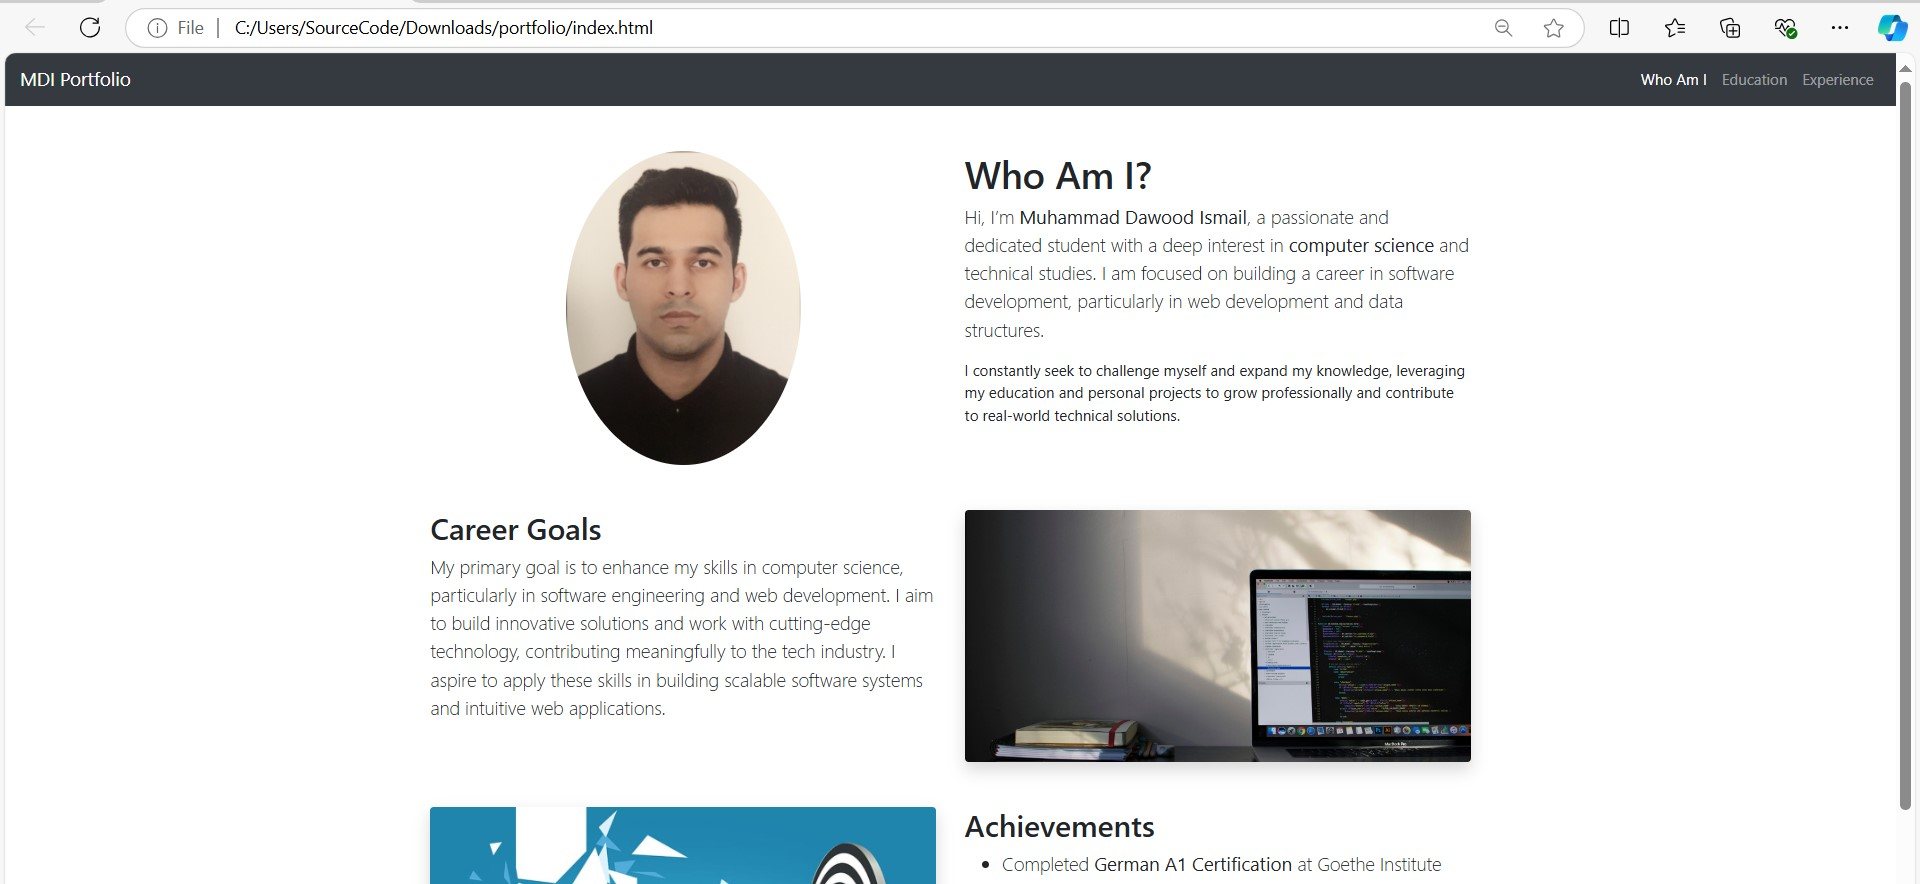
\includegraphics[width=0.8\textwidth]{index.jpg} % Replace with actual image path
    \caption{index page}
\end{figure}

\paragraph{Education Page}
The Education Page is clean and accessible, with my academic and technical background. Used Bootstrap's grid system to present details of education in a chic manner; it shows one section dedicated to certifications and another depicting academic achievements. Images have been provided for proper visualization of my educational journey. The visual aspect not only enhances the whole overview of the page, but it makes it more interactive removing the monotony of text and showing an interesting view. The information is brought forth with minimalism in mind so that the viewer gets quite clear.

\begin{figure}[h!]
    \centering
    
\includegraphics[width=0.8\textwidth]{education.jpg} % Replace with actual image path
    \caption{education page}
\end{figure}

\paragraph{Experience Page}
The Experience Page lists my technical projects and internships with short and concise descriptions of every project, including the technologies applied. Using images together with detailed project descriptions enables the visitor to perceive the scope and scale of the work executed. This power combination of visuals and text will give an immersive experience to show both the practical and technical aspects of my projects. The layout is the same as for the rest of the website, so that one could browse through easily, but it also will give a bit of an insight into my professional experience.

\begin{figure}[h!]
    \centering
    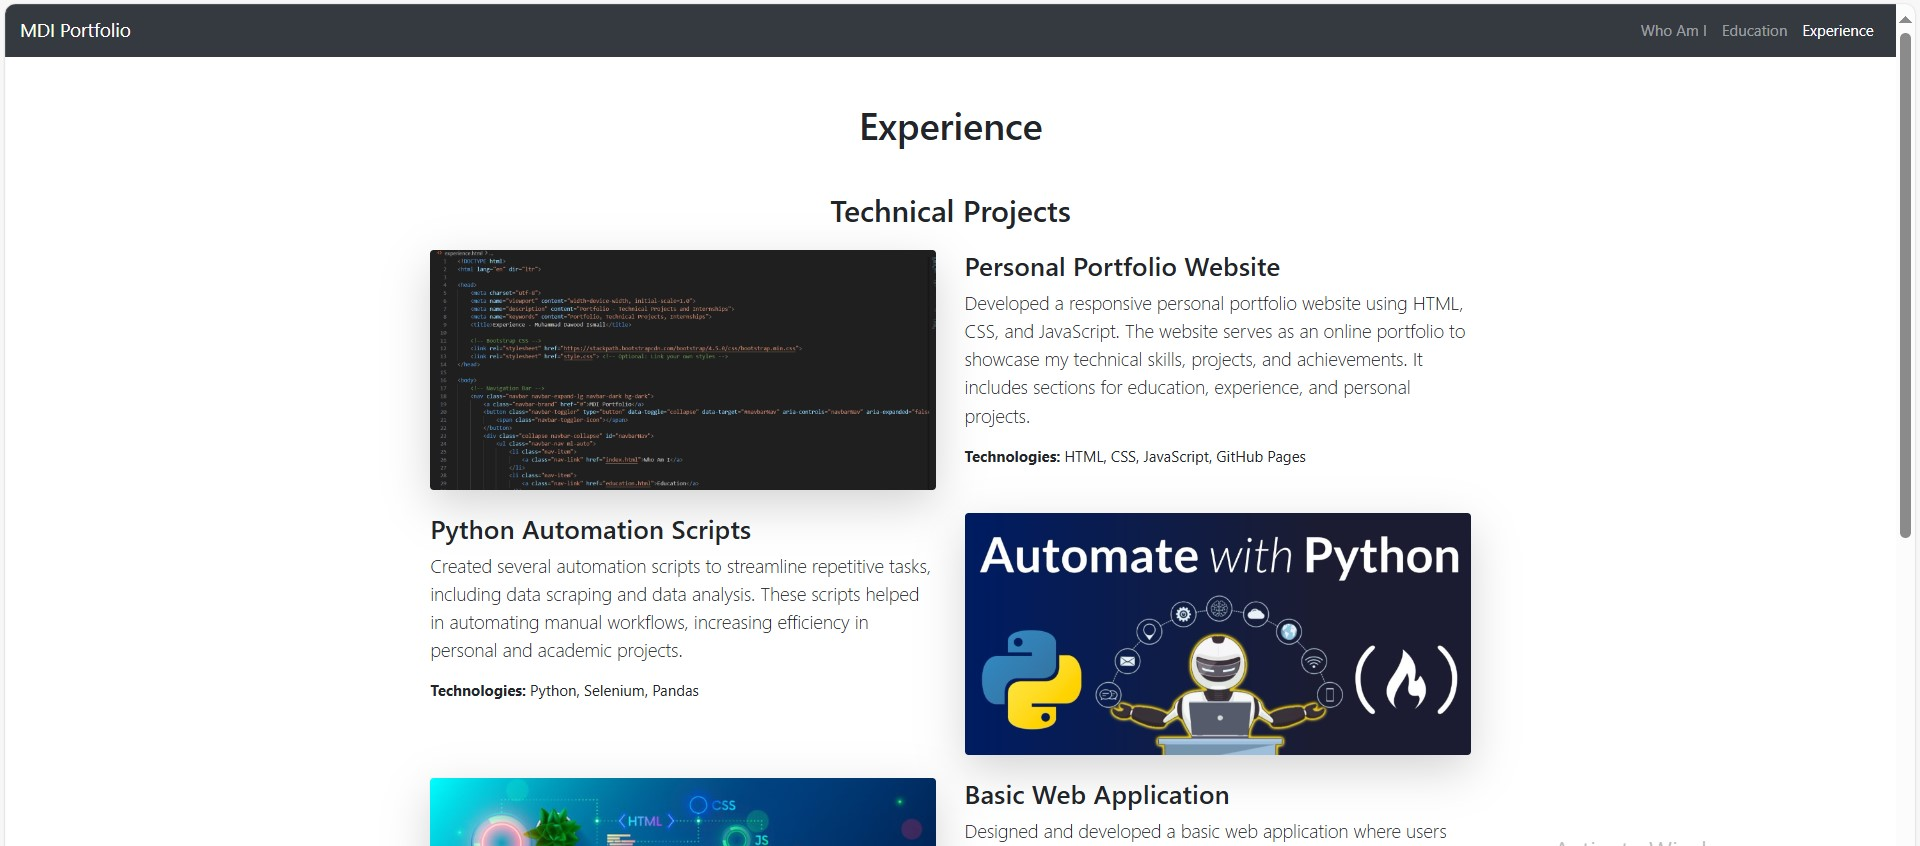
\includegraphics[width=0.8\textwidth]{experience.jpg} % Replace with actual image path
    \caption{experience page}
\end{figure}

% Subsubsection 2.1.2: Responsiveness of the Website
\subsubsection{Responsiveness of the Website}
The site will be fully responsive, able to adapt to various screen sizes and devices. It will provide the best user experience when this website is viewed from desktops, tabs, or smartphones. This is very important in responsiveness with Bootstrap's grid system, where content can flow freely according to the dimension of a device. Responsive images, flexible grids, and adjustable text sizes ensure that no single structural change visually or functionally breaks the layout of the website on any platform. This responsiveness only adds to the professionalism of my portfolio and validates the fact that I am attentive down to the smallest details when working with web development.

% Subsection 2.2: Design Decisions
\subsection{Design Decisions}
That would be economically expressed through the minimalist approach in readability and professional look used in designing the portfolio website. The design adopts a dark background and white for the text, ensuring high contrasting that promotes the readability of the text on any device. This combination is associated with professionalism and sophistication; thus, the website will look clean and more modern. The selection of simple and pretty fonts reinforces this minimalist theme really well, as it executes it so the subject is not overwhelmed by too much design element excess, hence the content is in focus. Overall, this line color and font selection brings the interface to end-users rather friendly, balancing between visualization and functionality.
The navigation would present the ease of moving through the website, intuitively and logically, by placing it on the top of the page using the Bootstrap framework for responsiveness. In the navigation bar, there are links provided to major sections like "Home," "Education," and "Experience." Every link is suitably labeled to answer the user's needs for quick access to the relevant content. The collapsible menu means that navigation is available not only on big screens but even on mobile, which enhances the user experience. Such easy and well-structured navigation adds to the overall usability of the website, ensuring ease for its visitors to explore its contents.
Images and media provide important contextualization, fleshing out a site visually and adding context to the content. Images can be found scattered throughout the site, as visualizations on skills, achievements, and projects. Technical project images also populate the "Experience" section in order to provide reinforcing visuals for the written description of each project. Notice how images and text are inclined together to make the experience for the visitor more immersive, drawing in and helping them understand the breadth and complexity of the represented work. Images also help break up some of the heavier sections of text on the site, making it more interesting and visually appealing.
HTML was used for structural development, CSS for styling purposes, and JavaScript for interactivity on the website. As a reason for choosing them, these languages are flexible and somehow easy to work with, in that one can nicely develop and customize the site with their efficiency. GitHub Pages were chosen to host this website because of their smooth integration with version control, affording an efficient and free method of maintaining and updating the site. It thereby allows one to create a light website based on both design and functionality, using technologies that will ensure smooth workflow while not compromising technical skills in web development.


% Subsection 2.3: Tools and Technologies
\subsection{Tools and Technologies}
Therefore, the Bootstrap framework was decided upon because of its keen capability concerning responsive design. It made the job of quick prototyping in website layout easier. Moreover, Bootstrap's grid allows for flexible and dynamic layouts; this means the website will seamlessly adapt to different screen sizes and devices. In other words, it ensures that users on both desktops and mobile devices will have the same experience as far as functionality is concerned. Moreover, with the great number of ready-to-use Bootstrap components, like navigation bars, buttons, and forms, the development is way too accelerated, permitting this professional site to be created in such an aesthetic manner.

% Subsection 2.5: Strengths and Weaknesses
\subsection{Strengths and Weaknesses}

\begin{table}[h!]
\centering
\begin{tabular}{|c|c|c|}
\hline
\textbf{Aspect} & \textbf{Strengths} & \textbf{Weaknesses} \\ \hline
Navigation & Clear and intuitive & Limited interactivity \\ \hline
Responsiveness & Fully responsive & Optimize image loading \\ \hline
Aesthetics & Professional aesthetic & Lack of media engagement \\ \hline
Technical Skills & Proficiency in HTML, CSS, Bootstrap & Needs dynamic features \\ \hline
Future Opportunities & Easy to expand & No real-time updates \\ \hline
\end{tabular}
\caption{Strengths and Weaknesses of the Website}
\end{table}

% Section 3: LaTeX CV
\section{LaTeX CV}

% Subsection 3.1: Document Overview
\subsection{Document Overview}
The LaTeX typeset CV is an integral part of my portfolio, reflecting both professionalism and technical skills. LaTeX is known for clearness and well-structured documents, a factor that presents a critical advantage in the technical area when precision and clarity mean everything. I managed to use LaTeX to develop a neat, well-structured, visually attractive CV, well-representing my qualifications. LaTeX has great formatting capabilities that provide uniform layout; therefore, the presentation of my CV is readable and professional, particularly about the technicalities of education and skills.

% Subsection 3.2: Design and Structure
\subsection{Design and Structure}
My key sections, which give an overview of my background and abilities within my CV, start with personal information and contact details, and afterwards, the sections related to education and certifications include the description of my academic history. Further, I have mentioned a Technical skills section encompassing my proficiency in programming languages and tools: Python, Java, and Git. The CV also includes a very elaborate description of my projects and work experiences that show how the skills could be applied to real-world practices. To achieve this structure, LaTeX packages used were fontawesome for icons to give an appealing look and geometry for margin management to make it professional and polished.

\begin{figure}[h!]
    \centering
    \includegraphics[width=0.8\textwidth]{cv.png} % Replace with actual image path
    \caption{LaTeX CV}
\end{figure}

% Section 4: Analytics Task
\section{Analytics Task}

% Subsection 4.1: Task Overview
\subsection{Task Overview}
The portfolio analytics task is designed to show my ability in manipulating data analysis using any programming language, but most especially Python. The aim here is to get a real-world dataset and analyze it using various techniques that have been covered in the course in data manipulation and visualization so as to come up with meaningful insights. This project will help me prove my skills in cleaning, processing, and visualizing data by implementing technical competencies in programming and data science. The analysis also affirms my understanding of machine learning models and their application in decision-making processes.

% Subsection 4.2: Dataset and Tools
\subsection{Dataset and Tools}
The dataset that will be used in this analysis pertains to the status of loan approval based on credit score, income, employment status, etc. This dataset has been chosen because it is highly applicable in a real-world environment, whereby a company needs to make financial decisions on the basis of loan applicants' varied and multi-factorial nature. In such a dataset, the diversity allows the exploration of data trends with model performance evaluation.
In this work, based on the following key libraries, data cleaning and final manipulation were done using Python: Pandas for cleaning and manipulating data, Matplotlib and Seaborn for visualization, and Scikit-learn for the implementation of machine learning models. These tools are quite efficient with regard to handling workflows in data and expressing their output in clear visuals, so they fit well for the task.


% Subsection 4.3: Analysis and Results
\subsection{Analysis and Results}
After dealing with missing values and restructuring all the variables in formats appropriate for analysis, even outliers were checked and treated appropriately. As and when the data was ready, I started with exploratory data analysis or EDA towards initial inspection of the loan statuses distribution and other important features. Graphs were made, including a bar chart to display the number of Y's. The second figure below depicts this.
Following the EDA, I used machine learning models to predict the status of whether a loan would be approved. I trained three models: Logistic Regression, Decision Tree, and Random Forest, and tested their performances for accuracy. From the first figure below, one can observe that the Random Forest model had the highest accuracy, closely followed by the Decision Tree model. This evidences my ability to use different machine learning models and compare their respective model performances in making predictions. The task allowed me to exploit my skills in data analysis, visualization, and predictive modeling relevant for solving a real-world problem with data-driven approaches.


\begin{figure}[h!]
    \centering
    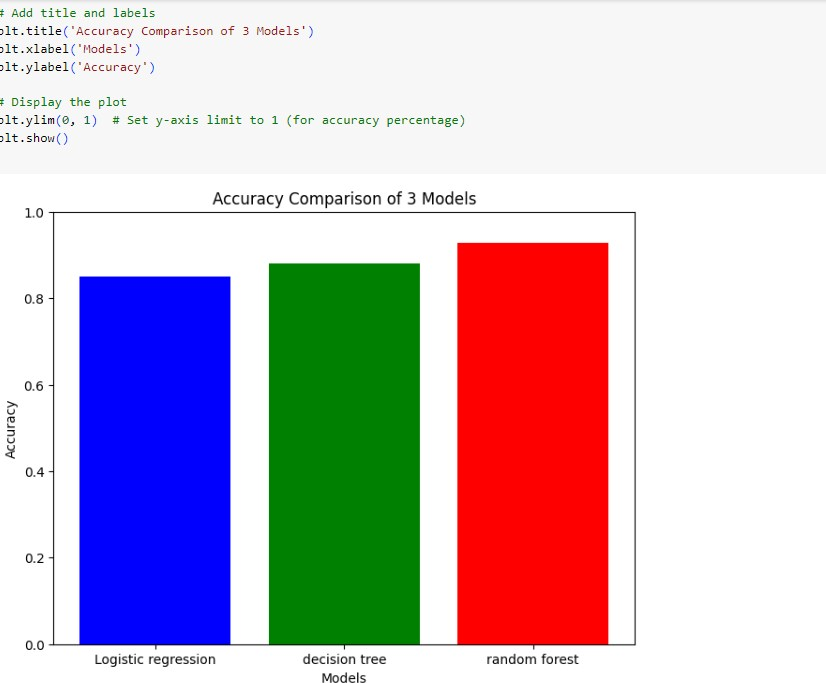
\includegraphics[width=0.8\textwidth]{results.jpg} % Replace with actual image path
    \caption{Python Results}
\end{figure}

% Section 5: Conclusion
\section{Conclusion}
It has three important parts showcasing my technical skills: the website, LaTeX CV, and analytics task. The website is a professional, organized way of representing my academic background, technical projects, and skills in graphical form. The website has utilized responsive design, clear navigation, and modern web development tools such as Bootstrap, HTML, and CSS for effective presentation and demonstration of my Web Development skills. This is a neat, professional LaTeX CV, which focuses on achievements, both academic and technical skills, and working experiences in a way that demonstrates precision and attention to detail. The analysis task depicts my skill in data analysis and machine learning with Python, where I applied techniques like cleaning the data, visualizing it, and evaluating models to derive insights from the real-world dataset.
Throughout the whole development process, I enriched myself with technical skills that perfectly meet the expectations of working students. The development of the website improved my knowledge of web development frameworks, while the creation of the LaTeX CV enforced my ability to present technical information in a clear and professional way. The analytics task that followed helped me further develop problem-solving skills and data processing abilities, giving me an important foundation for various analytical thinking-related job positions. This project generally helped me firm up the necessary technical knowledge: coding, design, analysis, and documentation.
Looking ahead, there is obviously potential for improvement in many aspects that could be improved upon in an ongoing way. I would also like to add a lot more interactive stuff on the site and probably include blogger features whereby I could share my updates on any ongoing projects or use advanced features of JavaScript. Regarding the CV, it would be updated with more up-to-date projects and certifications as one progresses in one's career. Regarding the analytics task, my key objective is working out advanced analytics approaches, such as the building of machine learning models beyond the classification tasks-perhaps even predictive forecasting or clustering-and ultimately really continuous analysis. This will be great value addition for my portfolio, too, and helps me continue my development regarding technical skills.



\end{document}
